
% \begin{figure*}[htbp]
%     \centering
%     \subfloat[\label{fig:subgenuscounts}]{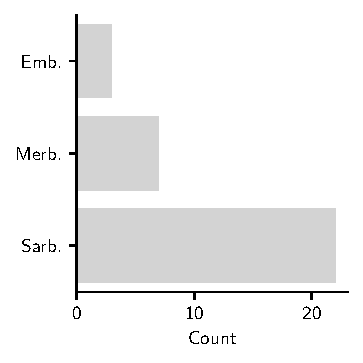
\includegraphics[height=5cm]{img/subgenus_counts.pdf}}
%     \subfloat[\label{fig:receptorcounts}]{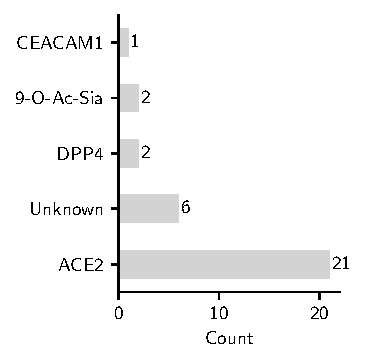
\includegraphics[height=5cm]{img/receptor_counts.pdf}}
%     \subfloat[]{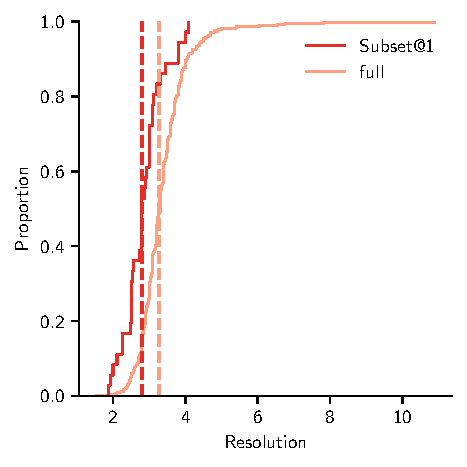
\includegraphics[height=5cm]{img/resolution_ecdf.pdf}}
%     \\
%     \begin{minipage}[b]{0.7\textwidth}
%         \subfloat[AA \label{fig:cons_aa}]{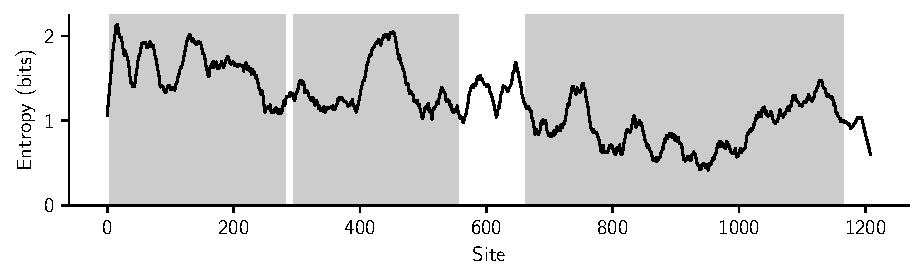
\includegraphics[height=3.8cm]{img/cons_aa.pdf}} \\
%         \subfloat[3Di \label{fig:cons_3di}]{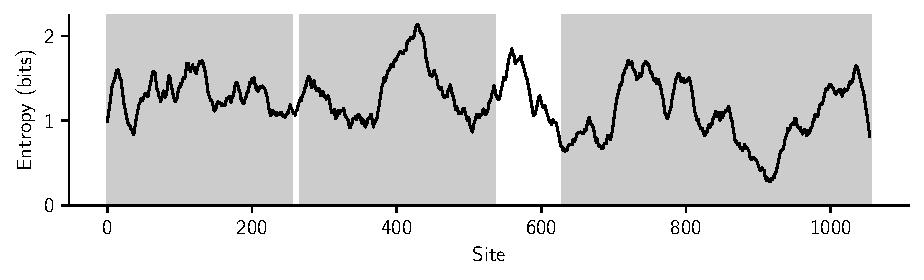
\includegraphics[height=3.8cm]{img/cons_3di.pdf}} 
%     \end{minipage}
%     \begin{minipage}[b]{0.27\textwidth}
%         \subfloat[\label{fig:cons_violin}]{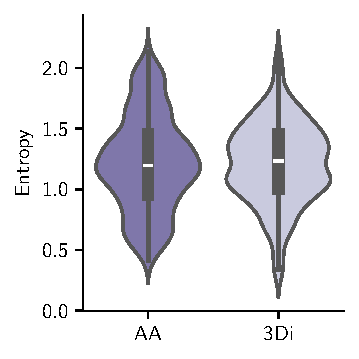
\includegraphics[height=3.8cm]{img/cons_violin.pdf}}
%         \\
%         \subfloat[\label{fig:cons_boot}]{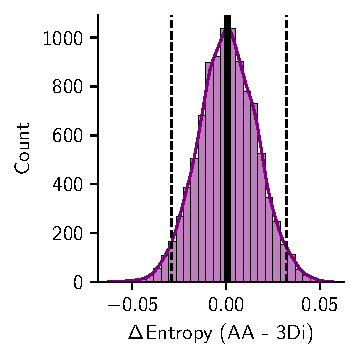
\includegraphics[height=3.8cm]{img/cons_bootstrap.pdf}}
%     \end{minipage}
%     \caption{Overview of the amino acid (AA) and 3Di-based alignments of 36 \textit{Betacoronavirus} spike glycoproteins. \textbf{(a)} \textit{Betacoronavirus} subgenus distribution in the dataset. Sarb.: \textit{Sarbecovirus}; Merb.: \textit{Merbecovirus}; Emb.: \textit{Embecovirus}. \textbf{(b)} Receptor distribution. CAECAM1: Carcinoembryonic antigen-related cell adhesion molecule 1. 9-O-Ac-Sia: 9-O-acetylated sialic acid. DPP4: Dipeptidyl peptidase-4 inhibitor. ACE2: angiontensin-converting enzyme 2. \textbf{(c)} Distribution of protein structure resolution in the full dataset (2,113 structures) and in the final dataset (`Subset@1`; 36 structures) used for downstream phylogenetic analyses. \textbf{(d, e)} Site-wise Shannon entropy of the amino acid (\textbf{(d)}) and structural (\textbf{(e)}) alignments. Shaded areas represent three domains of the S1 subunit (NTD, RBD, CTD), and the S2 subunit, inferred via InterProScan~\cite{jones2014}. \textbf{(f)} Distribution of site-wise in \textbf{(d)} and \textbf{(e)}. \textbf{(g)} Bootstrapped differences in site-wise entropy between the AA and 3Di dataset. Dashed lines denote the lower and upper bounds of the bootstrapped 95\% confidence interval, whereas the thicker line represents the mean. Reproduced from Scheidwasser \textit{et al.} (Ref.~\cite{scheidwasser2025a}), licensed under a Creative Commons Attribution License.}
%     \label{fig:bcov3d_subset1}
% \end{figure*}


% Finally, we intersected the obtained 3Di and \gls{aa} sequence sets and retained one representative sequence per virus, except for SARS-CoV-2, for which we selected one sequence per major variant (Alpha, Delta, Omicron, wild type) and one sequence representing other variants (e.g., Beta, Kappa, Eta). For each virus and/or major variant, the representative sequence was the least gappy sequence of its group. The obtained subset comprised 36 sequences spanning three subgenera of betacoronaviruses (\textit{Sarbecovirus, Merbecovirus, Embecovirus}) which bind to various target receptors: angiotensin-converting enzyme 2 (ACE2), dipeptidyl peptidase-4 inhibitors (DPP4), and N-acetyl-9-O-acetylneuraminic acid receptors.



% Second, we aligned the filtered sequences using \texttt{MAFFT} with the \texttt{auto} and \texttt{leavegappyout} arguments, using the scoring matrix computed by Van Kempen \textit{et al.}~\cite{vankempen2024}. Gappy sites were trimmed from the aligned sequences using \texttt{trimal} (v1.5.rev0)~\cite{capella2009} with a gap threshold of 50\% (i.e., sites with gaps in 50\% or more of the sequences are removed). Finally, duplicate sequences were removed, yielding a set of 615 sequences.

% Third, we processed the amino acid sequences from the deduplicated 3Di set. Similar to the 3Di pipeline, we used \texttt{MAFFT} and \texttt{trimal} for alignment and site trimming, respectively. The same parameters were used, except for the scoring matrix, where BLOSUM62~\cite{henikoff1992} was used. Additionally, we removed sequences with 50\% or more gaps in the alignment and ran a similar sequence deduplication process, yielding a set of 263 sequences.